\section{Introduction}

Graph data pervade numerous domains such as social networks, biological systems, recommendation engines, and e-commerce networks~\cite{zhang2020deep, wu2020comprehensive}.
The graph is well-suited for modeling complex real-world relationships.

Predicting missing or potential connections within a graph is essential for many applications, unlocking valuable insight and facilitating intelligent decision-making. 
The ability to predict future network interactions can be applied to diverse domains, including friend recommendations on social networks~\cite{adamic2003friends, yao2016link, fire2011link}, knowledge graph completion~\cite{kazemi2018simple, nayyeri2021link}, identification of potential drug-protein interactions in bioinformatics~\cite{stanfield2017drug, nasiri2021novel}, prediction protein interactions~\cite{lei2013novel, kovacs2019network, nasiri2021novel}, and optimization of supply chain logistics~\cite{brockmann2022supply, brintrup2018predicting}.

The link prediction (LP) problem has been categorized into three major paradigms: heuristic methods, embedding methods, and graph neural network (GNN)-based methods, which are explored in detail in Section~\ref{sec:related works}.
Recently, compared to heuristic~\cite{adamic2003friends, lu2011link, barabasi1999emergence, zhou2009predicting, brin2012reprint, jeh2002simrank} and embedding methods~\cite{koren2009matrix, perozzi2014deepwalk, grover2016node2vec, tang2015line}, GNN-based models have achieved significant score improvements in capturing intricate relationships within graphs~\cite{kipf2016variational, zhang2018link, yun2021neo, mavromatis2020graph, yan2021link, pan2021neural}. 

However, GNN-based methods are comprised of neural networks, making it challenging to understand the reasons for their performance.
To explore these reasons, we employ persistent homology (PH), a mathematical tool in topological data analysis (TDA) that enables the inference of topological information regarding the manifold approximating the data~\cite{huber2021persistent, dey2022computational} by quantifying the persistence of topological features across multiple scales.
Various research has had successful outcomes in applying PH to graph classification and node classification tasks~\cite{horn2021topological, ye2023treph, carriere2020perslay, taiwo2024explaining, wen2024tensor, immonen2024going, ying2024boosting, zhao2019learning, chen2021topological, zhao2020persistence}.
In contrast, relatively few studies have explored using PH for LP.
The topological loop-counting (TLC) GNN~\cite{yan2021link} is a notable example that uses PH.
The TLC-GNN injects topological information into a GNN, and experiments were conducted on benchmark data where node attributes are available.


\begin{figure}[!t]
\centering
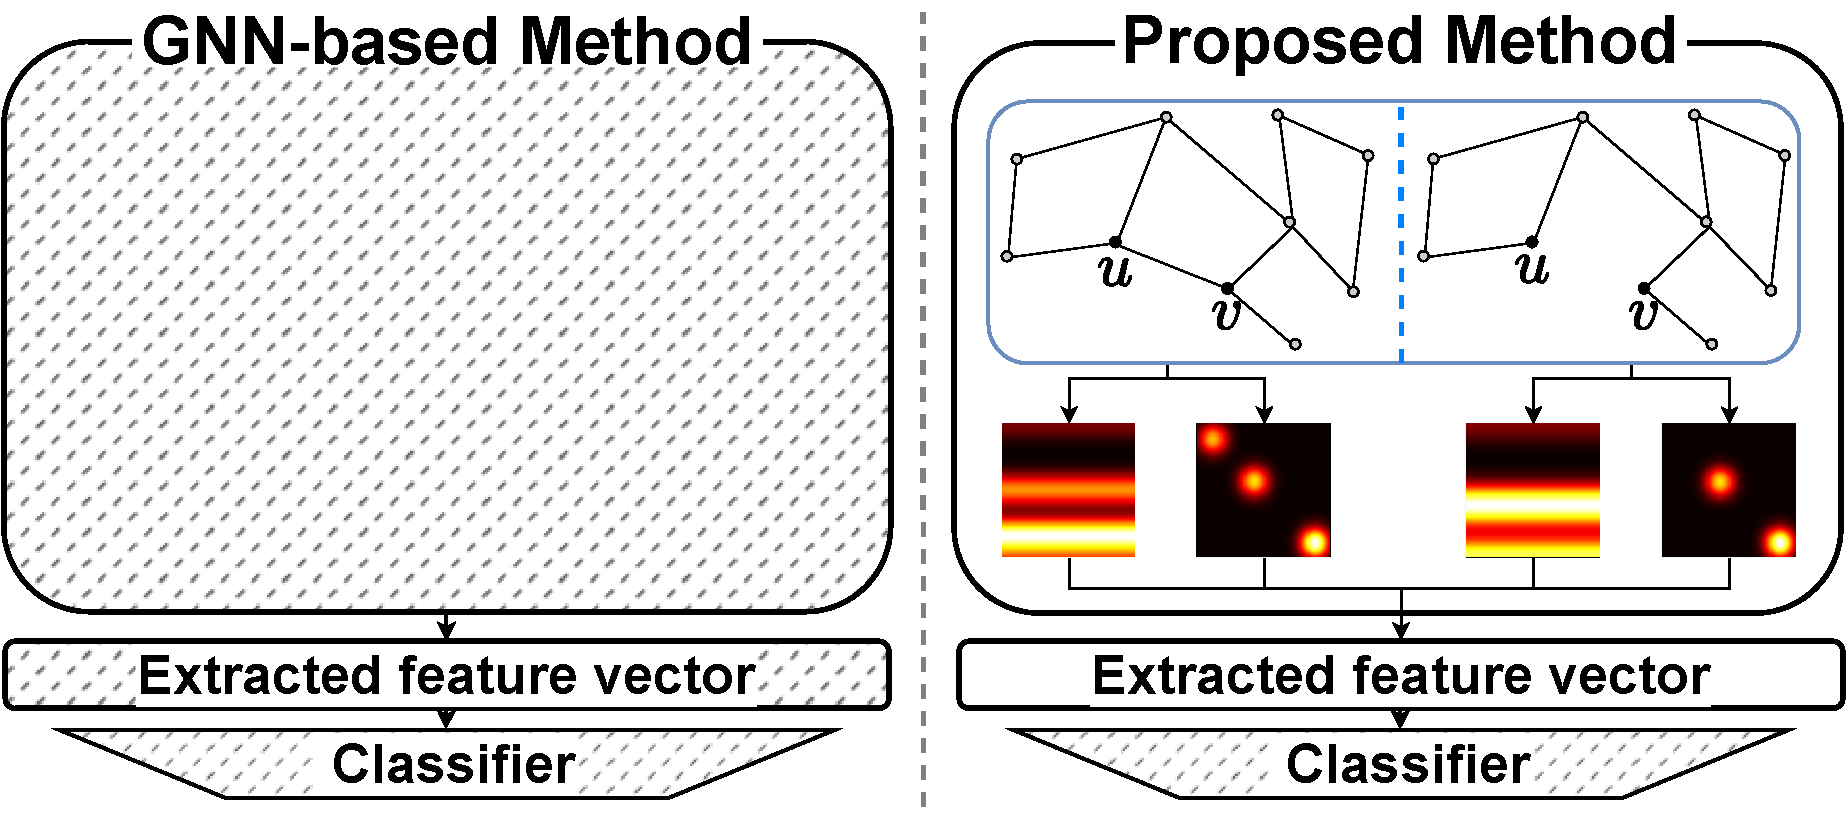
\includegraphics[width=\linewidth]{figures/Blackbox.drawio.pdf} 
\caption{ Difference between the GNN-based and proposed methods.
(Left) The GNN-based method extracts feature vectors through optimization (dashed area), making it difficult to interpret what these vectors represent. (Right) The proposed method extracts feature vectors through the designed analysis process, resulting in interpretable vectors.}
\label{fig:Blackbox}
\end{figure}

\begin{figure*}[!htbp]
\centering
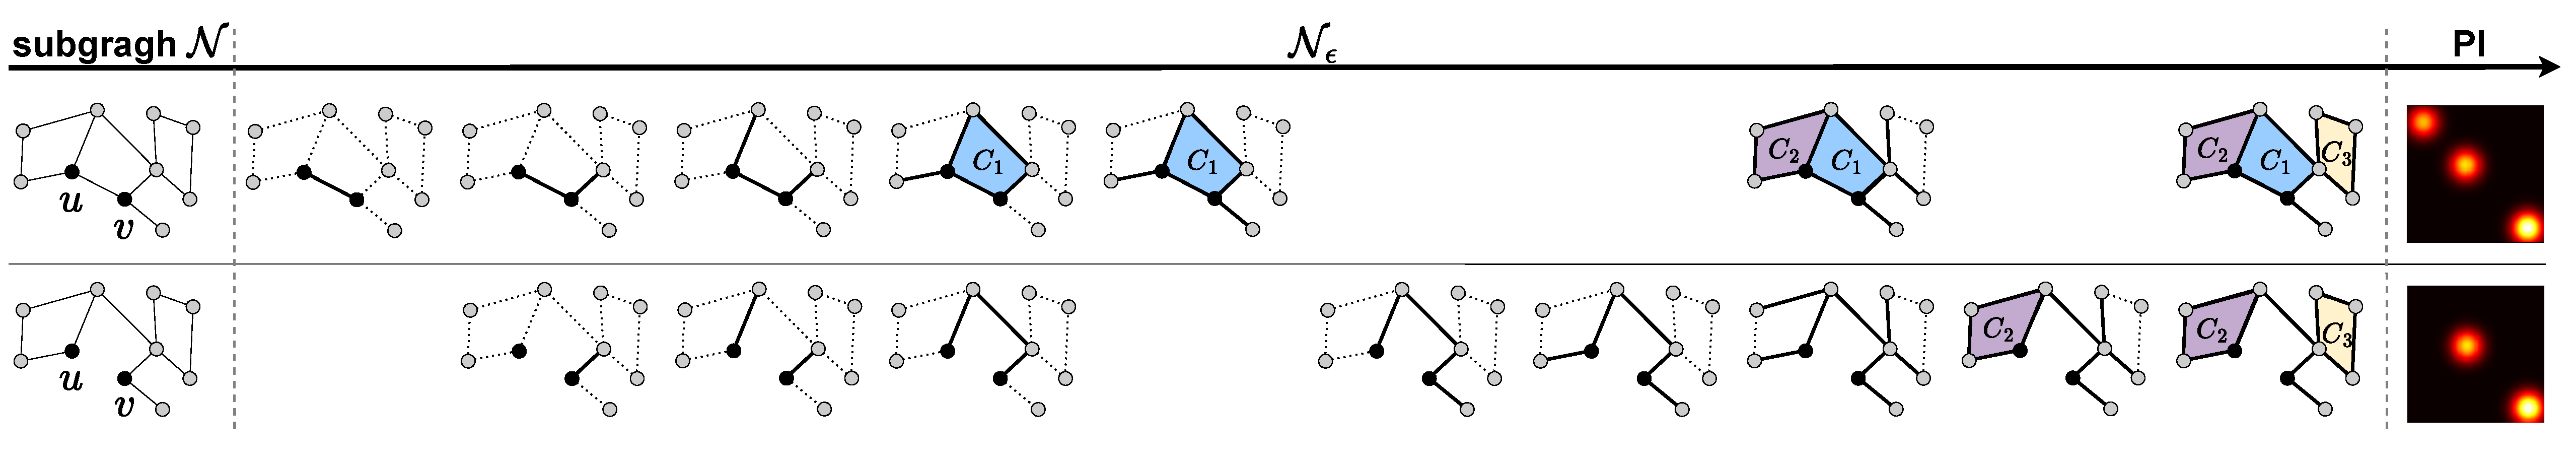
\includegraphics[width=\linewidth]{figures/Filtraion.intro.pdf}
\vspace{-7mm}
\caption{Topological features in subgraphs with and without a target link $(u,v)$.
The diagram illustrates the topological information extraction process for the subgraph $\mathcal{N}$, as described in Section~\ref{subsec:persistenthomology}. 
The presence (top) or absence (bottom) of the target link changes the topological structure of the graph. 
Top row: When the target link is connected, three features ($C_1$, $C_2$, and $C_3$) are detected shown in the persistence image (PI) in the right column.
The PI represents the topological features of the subgraph $\mathcal{N}$ (Section~\ref{subsec:persistenceimage}).
Bottom row: When the target link is absent, only two features ($C_2$ and $C_3$) are detected as depicted in the corresponding PI. }
\label{motivation}
\end{figure*}

In this context, as illustrated in Fig.~\ref{fig:Blackbox}, we present a novel approach to LP, called PHLP, which calculates the topological information of a graph.
To use the topological information of subgraphs for LP, we measure how the topological information changes depending on the existence of the target link, as illustrated in Fig.~\ref{motivation}.
To extract topological information from various perspectives, we utilize \textit{angle hop subgraphs} for each target node. 
Additionally, we propose new node labeling called \textit{degree double radius node labeling (Degree DRNL)}, which incorporates degree information for each node, using DRNL~\cite{zhang2018link}.

The contributions are summarized as follows:
\begin{itemize}
    \item We develop an explainable LP method, PHLP, that employs the topological information for LP through PH without relying on neural networks, as illustrated in Fig.~\ref{fig:Blackbox}.
    \item We demonstrate that the proposed method, even with a simple classifier such as a multilayer perceptron (MLP), can achieve LP performance close to that of state-of-the-art (SOTA) models.
    This method surpassed the SOTA performance for the Power dataset.
    \item We reveal that merely incorporating vectors computed by PHLP into existing LP models, including SOTA models, can improve their performance.
    \item To the best of our knowledge, the proposed method using PH without a GNN is the first to achieve performance close to that of SOTA models.
\end{itemize}